% ===================================================================
%  Week 12 — From Image Features to Machine Learning
% ===================================================================
\documentclass[10pt,aspectratio=169]{beamer}
% ===================================================================
%  Shared Beamer preamble for "Practical Image Processing"
%  English slides. Compile with pdfLaTeX.
% ===================================================================

\usetheme{metropolis}
\usepackage[T1]{fontenc}
\usepackage[utf8]{inputenc}
\usepackage{lmodern}
\usepackage{listings}
\usepackage{tcolorbox}
\usepackage{fontawesome5}
\usepackage{booktabs}
\usepackage{amsmath,amssymb}
\usepackage{tikz}
\usepackage{pgfplots}
\pgfplotsset{compat=1.17}
\usetikzlibrary{arrows.meta,positioning,shapes.geometric,fit,backgrounds,matrix}
\tcbuselibrary{skins,breakable}

% ---- Palette --------------------------------------------------------
\definecolor{coursePrimary}{HTML}{1B4965}   % deep blue
\definecolor{courseAccent}{HTML}{E76F51}    % coral
\definecolor{courseGood}{HTML}{2A9D8F}      % teal
\definecolor{courseBad}{HTML}{C0392B}       % red
\definecolor{courseInfo}{HTML}{2980B9}      % blue
\definecolor{codeBg}{HTML}{F5F6FA}
\definecolor{codeKw}{HTML}{8E44AD}
\definecolor{codeStr}{HTML}{2A9D8F}
\definecolor{codeCom}{HTML}{7F8C8D}

\setbeamercolor{frametitle}{bg=coursePrimary}
\setbeamercolor{progress bar}{fg=courseAccent}
\setbeamercolor{alerted text}{fg=courseAccent}
\metroset{block=fill,sectionpage=progressbar,numbering=fraction}

% ---- Code listings (Python is built into listings) -----------------
\lstdefinestyle{course}{
  backgroundcolor=\color{codeBg},
  basicstyle=\ttfamily\scriptsize,
  keywordstyle=\color{codeKw}\bfseries,
  stringstyle=\color{codeStr},
  commentstyle=\color{codeCom}\itshape,
  numberstyle=\tiny\color{codeCom},
  numbers=left, numbersep=6pt,
  showstringspaces=false, breaklines=true, breakatwhitespace=true,
  tabsize=4, columns=fullflexible,
  frame=single, framesep=4pt, rulecolor=\color{gray!30},
  keepspaces=true, upquote=true, language=Python,
}
\lstset{style=course}
\lstdefinelanguage{bash}{
  keywords={cd,pip,python,venv,source,import}, sensitive=true,
  morecomment=[l]{\#}, morestring=[b]', morestring=[b]",
}

% ---- Reusable callout boxes ----------------------------------------
\newtcolorbox{goodbox}[1][Good practice]{colback=courseGood!8,colframe=courseGood,
  fonttitle=\bfseries,title={\faCheck~#1},boxrule=0.6pt,left=4pt,right=4pt,top=3pt,bottom=3pt}
\newtcolorbox{badbox}[1][Pitfall]{colback=courseBad!8,colframe=courseBad,
  fonttitle=\bfseries,title={\faTimes~#1},boxrule=0.6pt,left=4pt,right=4pt,top=3pt,bottom=3pt}
\newtcolorbox{infobox}[1][Note]{colback=courseInfo!8,colframe=courseInfo,
  fonttitle=\bfseries,title={\faInfoCircle~#1},boxrule=0.6pt,left=4pt,right=4pt,top=3pt,bottom=3pt}
\newtcolorbox{mathbox}[1][Math]{colback=coursePrimary!6,colframe=coursePrimary,
  fonttitle=\bfseries,title={\faCalculator~#1},boxrule=0.6pt,left=4pt,right=4pt,top=3pt,bottom=3pt}

\newcommand{\keyidea}[1]{\begin{alertblock}{Key idea}#1\end{alertblock}}
\newcommand{\term}[1]{\textbf{\color{coursePrimary}#1}}
\newcommand{\code}[1]{\lstinline[basicstyle=\ttfamily\small]|#1|}

% ---- A helper to draw a small pixel grid, cells shaded by value ----
% \pixelgrid{ {10,20,120,200,240}, {30,60,130,180,230}, ... }
\newcommand{\pixelgrid}[1]{%
  \begin{tikzpicture}[font=\scriptsize,scale=0.6]
    \foreach \row [count=\ry] in {#1} {
      \foreach \val [count=\cx] in \row {
        \draw[gray,fill=coursePrimary!8] (\cx,-\ry) rectangle ++(1,-1);
        \node at (\cx+0.5,-\ry-0.5) {\val};
      }
    }
  \end{tikzpicture}}


\title{From Features to Machine Learning}
\subtitle{Week 12 — Turning image features into a classifier}
\author{Practical Image Processing}
\date{Lecture 12 \textbullet\ 60--70 min}

\begin{document}

\maketitle

\begin{frame}{A turning point in the course}
  \begin{columns}[T]
    \begin{column}{0.58\textwidth}
      \begin{itemize}
        \item Weeks 1--11: \emph{we} designed every step (filters, edges, corners, warps).
        \item \alert{Now:} we let the computer \emph{learn} the decision from labelled examples.
        \item The bridge: turn an image into a \term{feature vector}, then train a \term{classifier}.
      \end{itemize}
    \end{column}
    \begin{column}{0.42\textwidth}
      \begin{alertblock}{Today's real task}
        Classify Iranian car models (206 / 405 / Dena) from \term{HOG} features — using your
        \code{E:/data} images.
      \end{alertblock}
    \end{column}
  \end{columns}
\end{frame}

\begin{frame}{Roadmap}\tableofcontents\end{frame}

% ==================================================================
\section{The feature → classifier pipeline}
% ==================================================================

\begin{frame}{The classic recognition pipeline}
  \begin{enumerate}
    \item \term{Input image} $\rightarrow$
    \item \term{Feature extraction} (turn pixels into a compact vector) $\rightarrow$
    \item \term{Classifier} (a learned function vector $\rightarrow$ label) $\rightarrow$
    \item \term{Prediction} (206 / 405 / Dena).
  \end{enumerate}
  \keyidea{Until $\sim$2012, essentially all recognition worked this way. The features were hand-designed; only the classifier was learned.}
\end{frame}

\begin{frame}{Why not feed raw pixels?}
  \begin{itemize}
    \item A $96\times96$ image is 9216 numbers — huge, and every shift/lighting change moves them all.
    \item Raw pixels are not \term{invariant}: the same car, moved 5 px, looks ``different''.
    \item \term{Features} (HOG, colour histograms, ORB) compress the image into a stable, meaningful vector.
  \end{itemize}
  \begin{mathbox}
    Good features make classes \term{separable}: similar things land near each other in feature space.
  \end{mathbox}
\end{frame}

\begin{frame}{HOG: Histogram of Oriented Gradients}
  \begin{columns}[T]
    \begin{column}{0.5\textwidth}\begin{center}
      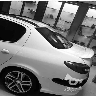
\includegraphics[width=0.8\linewidth]{../assets/sample_gray.png}\\{\scriptsize a real 206}
    \end{center}\end{column}
    \begin{column}{0.5\textwidth}\begin{center}
      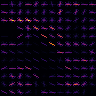
\includegraphics[width=0.8\linewidth]{../assets/hog_vis.png}\\{\scriptsize its HOG (edge-orientation) map}
    \end{center}\end{column}
  \end{columns}
  \vspace{2pt}
  HOG divides the image into cells and, in each, histograms the gradient directions — a compact shape signature.
\end{frame}

\begin{frame}{Why HOG works for shape}
  \begin{itemize}
    \item Cars differ in \emph{shape} (roofline, lights, grille) — captured by gradient directions.
    \item Histogramming per cell gives tolerance to small shifts and lighting changes.
    \item HOG + linear SVM was the state of the art for pedestrian/vehicle detection for years.
  \end{itemize}
  \keyidea{HOG throws away exact pixel values and keeps \emph{where edges point} — the essence of shape.}
\end{frame}

% ==================================================================
\section{Classifiers}
% ==================================================================

\begin{frame}{What a classifier learns}
  \begin{itemize}
    \item Given feature vectors with labels, it learns a \term{decision boundary} between classes.
    \item \term{k-NN}: label a point by the majority vote of its $k$ nearest training points.
    \item \term{SVM}: find the boundary with the widest \term{margin} between classes.
  \end{itemize}
  \begin{mathbox}
    k-NN memorizes; SVM optimizes a margin. Both need features where classes are separable.
  \end{mathbox}
\end{frame}

\begin{frame}{Our classes in feature space (PCA to 2D)}
  \begin{center}
  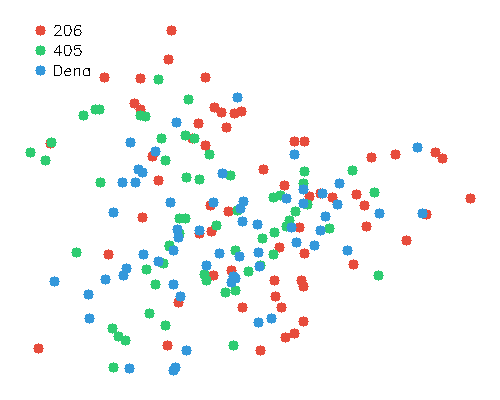
\includegraphics[width=0.5\linewidth]{../assets/feature_space.png}
  \end{center}
  \begin{itemize}
    \item Each dot is a real car's HOG vector, projected to 2D with PCA.
    \item Classes overlap a lot — these three models genuinely look similar. Hard problem!
  \end{itemize}
\end{frame}

\begin{frame}{Train / test split — the golden rule}
  \begin{itemize}
    \item Split data: \term{train} the classifier on one part, \term{test} on unseen data.
    \item Testing on training data lies — the model can just memorize.
    \item We used 70\% train / 30\% test, \term{stratified} (each class balanced in both).
  \end{itemize}
  \begin{badbox}
    Never report accuracy on data the model has seen. That number is meaningless for real use.
  \end{badbox}
\end{frame}

% ==================================================================
\section{Results \& overfitting}
% ==================================================================

\begin{frame}{Our real results (and an honest lesson)}
  \begin{center}
  \begin{tabular}{@{}lcc@{}}
    \toprule
    \textbf{Classifier} & \textbf{Train acc} & \textbf{Test acc} \\
    \midrule
    k-NN ($k{=}5$) & 0.65 & 0.43 \\
    SVM (RBF) & \alert{1.00} & \alert{0.48} \\
    \bottomrule
  \end{tabular}
  \end{center}
  \vspace{3pt}
  Chance is 0.33 (3 classes). Both beat chance — but the SVM scores \textbf{100\% on train, 48\% on test}.
  That gap is \term{overfitting}.
\end{frame}

\begin{frame}{Overfitting, explained}
  \begin{itemize}
    \item \term{Overfitting}: the model memorizes training quirks instead of the real pattern.
    \item Symptom: train accuracy $\gg$ test accuracy (here 1.00 vs 0.48).
    \item Cures: more data, simpler model, regularization, better/invariant features.
  \end{itemize}
  \keyidea{A model that is perfect on training data and mediocre on test data has learned the wrong thing.}
\end{frame}

\begin{frame}{Reading the confusion matrix}
  \begin{columns}[T]
    \begin{column}{0.5\textwidth}\begin{center}
      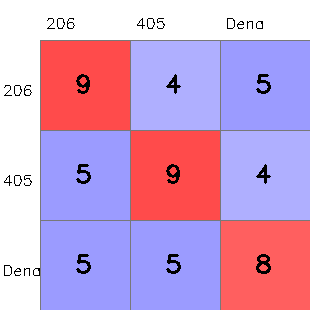
\includegraphics[width=0.95\linewidth]{../assets/confusion.png}
    \end{center}\end{column}
    \begin{column}{0.5\textwidth}
      \begin{itemize}
        \item Rows = true class, columns = predicted.
        \item Diagonal = correct; off-diagonal = the mistakes.
        \item Shows \emph{which} models get confused — far more useful than a single accuracy number.
      \end{itemize}
    \end{column}
  \end{columns}
\end{frame}

\begin{frame}{Metrics beyond accuracy}
  \begin{itemize}
    \item \term{Accuracy} hides imbalance: 95\% ``all normal'' is useless if 5\% are the faults you need.
    \item \term{Precision}: of predicted-positive, how many were right? \term{Recall}: of actual-positive, how many did we catch?
    \item \term{F1}: their harmonic mean. Report these per class, not one global number.
  \end{itemize}
  \begin{mathbox}
    Precision $=\dfrac{TP}{TP+FP}$,\quad Recall $=\dfrac{TP}{TP+FN}$,\quad F1 $=\dfrac{2\,PR}{P+R}$.
  \end{mathbox}
\end{frame}

% ==================================================================
\section{In-class exercise}
% ==================================================================

\begin{frame}{\faPen~In-class exercise (10 min)}
  \begin{infobox}[Diagnose the model]
  \end{infobox}
  \begin{enumerate}
    \item Our SVM got train 1.00, test 0.48. Name the problem and two ways to reduce it.
    \item A fault detector reports 96\% accuracy but faults are 4\% of data. Why might it be useless?
    \item You want to tell 206 from 405. What feature besides HOG might help separate them?
  \end{enumerate}
\end{frame}

\begin{frame}{\faPen~Debrief}
  \begin{itemize}
    \item (1) \term{Overfitting}: gather more data, simplify/regularize the SVM (lower $C$), or use better features.
    \item (2) Predicting ``no fault'' always scores 96\% but has \term{zero recall} on faults — accuracy is the wrong metric.
    \item (3) \term{Colour histograms} (models differ in typical colour), size/aspect, or logo region features.
  \end{itemize}
  \keyidea{A number without a train/test split and a confusion matrix tells you almost nothing.}
\end{frame}

% ==================================================================
\section{Deep dive}
% ==================================================================

\begin{frame}{Feature engineering vs feature learning}
  \begin{itemize}
    \item Today we \term{engineered} features (HOG) and learned only the classifier.
    \item The 48\% ceiling on look-alike cars hints at the limit of hand-designed features.
    \item \term{Deep learning} (Weeks 13--14) \emph{learns the features too}, directly from pixels.
  \end{itemize}
  \keyidea{The classical pipeline plateaus on hard, fine-grained problems. That plateau is exactly why CNNs took over.}
\end{frame}

\begin{frame}{Why our SVM overfit so hard}
  \begin{itemize}
    \item Only 126 training vectors, each 900-dimensional — far more features than examples.
    \item An RBF SVM with high $C$ can bend the boundary to fit every training point exactly.
    \item Result: train 1.00, but the boundary is tuned to noise $\rightarrow$ test collapses to 0.48.
  \end{itemize}
  \keyidea{More dimensions than samples is a red flag: the model has enough freedom to memorize. Reduce $C$, reduce dimensions (PCA), or get more data.}
\end{frame}

\begin{frame}{Cross-validation \& not fooling yourself}
  \begin{itemize}
    \item A single split is noisy. \term{k-fold cross-validation} averages over $k$ splits for a stable estimate.
    \item Tune hyper-parameters on a \term{validation} set (or CV) — never on the test set.
    \item The test set is used \emph{once}, at the very end. Peeking at it inflates your reported score.
  \end{itemize}
\end{frame}

\begin{frame}{Where this fits DocScan}
  \begin{itemize}
    \item DocScan must read digits. A digit is a small image; a classifier maps it to 0--9.
    \item Today's pipeline (features $\rightarrow$ classifier) is exactly how classic OCR worked.
    \item Next week we replace hand features with a \term{CNN} that learns them — and accuracy jumps.
  \end{itemize}
\end{frame}

\begin{frame}[fragile]{The whole ML pipeline in code}
\begin{lstlisting}[language=Python]
X = [hog(gray(img)) for img in images]      # features
Xtr, Xte, ytr, yte = train_test_split(X, y, test_size=0.3,
                                      stratify=y)
clf = SVC(kernel='rbf', C=10).fit(Xtr, ytr) # learn
print(accuracy_score(yte, clf.predict(Xte)))# HONEST score
print(confusion_matrix(yte, clf.predict(Xte)))
\end{lstlisting}
  Extract features $\rightarrow$ split $\rightarrow$ fit $\rightarrow$ evaluate on unseen data. Always in that order.
\end{frame}

% ==================================================================
\section{Wrap-up}
% ==================================================================

\begin{frame}{What you should now be able to do}
  \begin{itemize}
    \item Build a features $\rightarrow$ classifier pipeline (HOG + SVM/k-NN) on real images.
    \item Split train/test correctly and read a confusion matrix.
    \item Recognize overfitting (train $\gg$ test) and name cures.
    \item Explain why accuracy alone misleads, and when precision/recall matter.
  \end{itemize}
\end{frame}

\begin{frame}{This week's deliverable}
  \begin{alertblock}{Due before Week 13 (see \code{project/})}
    \begin{enumerate}
      \item Extract HOG features for 2--3 classes from \code{E:/data}; build $X, y$.
      \item Train k-NN and SVM with a stratified train/test split; report both accuracies.
      \item Show the confusion matrix; identify which classes get confused.
      \item Diagnose overfitting and try one cure; report whether the test score improved.
    \end{enumerate}
  \end{alertblock}
\end{frame}

\begin{frame}[standout]
  Features make it learnable; the split keeps you honest.\\[4pt]
  \normalsize Hand-designed features hit a ceiling — next week we learn the features themselves.
\end{frame}

\end{document}
